
% !TeX root = ../book.tex
% !TeX spellcheck = fr_FR
% !TeX encoding = ISO-8859-1

\section{Le r�tro qui double}\label{sec:B11}

C'est un r�tro violent qui faut utiliser avec discernement. Avec un
r�tro normal, nous sentons que la 2 nous �chappe, elle s'�carte ou bien
nous ne parviendrons pas � jouer suffisamment doucement pour � la fois
faire le point et ramener et garder la 2 pr�s de la 3. Avant de choisir
ce coup, v�rifions tout de m�me que la 2 ne s'�chappe pas trop loin....
En fait, celle-ci rentre presque sinon, la doubler nous la fera perdre
d�finitivement.

Prendre la 2 en r�tro pas trop bas en force, afin de donner un mouvement
de retour relativement lent � la 1 pendant que la 2 prend l'�nergie
suffisante pour parcourir 4 fois la largeur de la table. On esp�re que
la 2 reviendra dans le jeu, l'effet appliqu�, contraire � sa fuite,
devant la forcer � y rester.

Remarque : Il sera prudent de v�rifier que la 2 ne vient pas percuter la
1 avant de doubler, auquel cas, le r�sultat deviendrait al�atoire. Si
tel devait �tre le cas, on aurait d� choisir un r�tro simple, profitant
de la bosse pour ralentir la 2 et conserver une chance de regroupement.
Si la 2 rentre difficilement dans le jeu m�me apr�s deux retours, il
sera prudent avant toute d�cision, de v�rifier si un B simple sur la 3
n'est pas possible en attendant une position plus favorable.

R�fl�chissons avant de tenter ce coup... il semble facile quand on est
bien stable et horizontal mais la rentr�e convenable est souvent
impr�cise. Ce point constitue souvent un point d'attente et non de
construction.

\begin{figure}[htb]
	\centering
	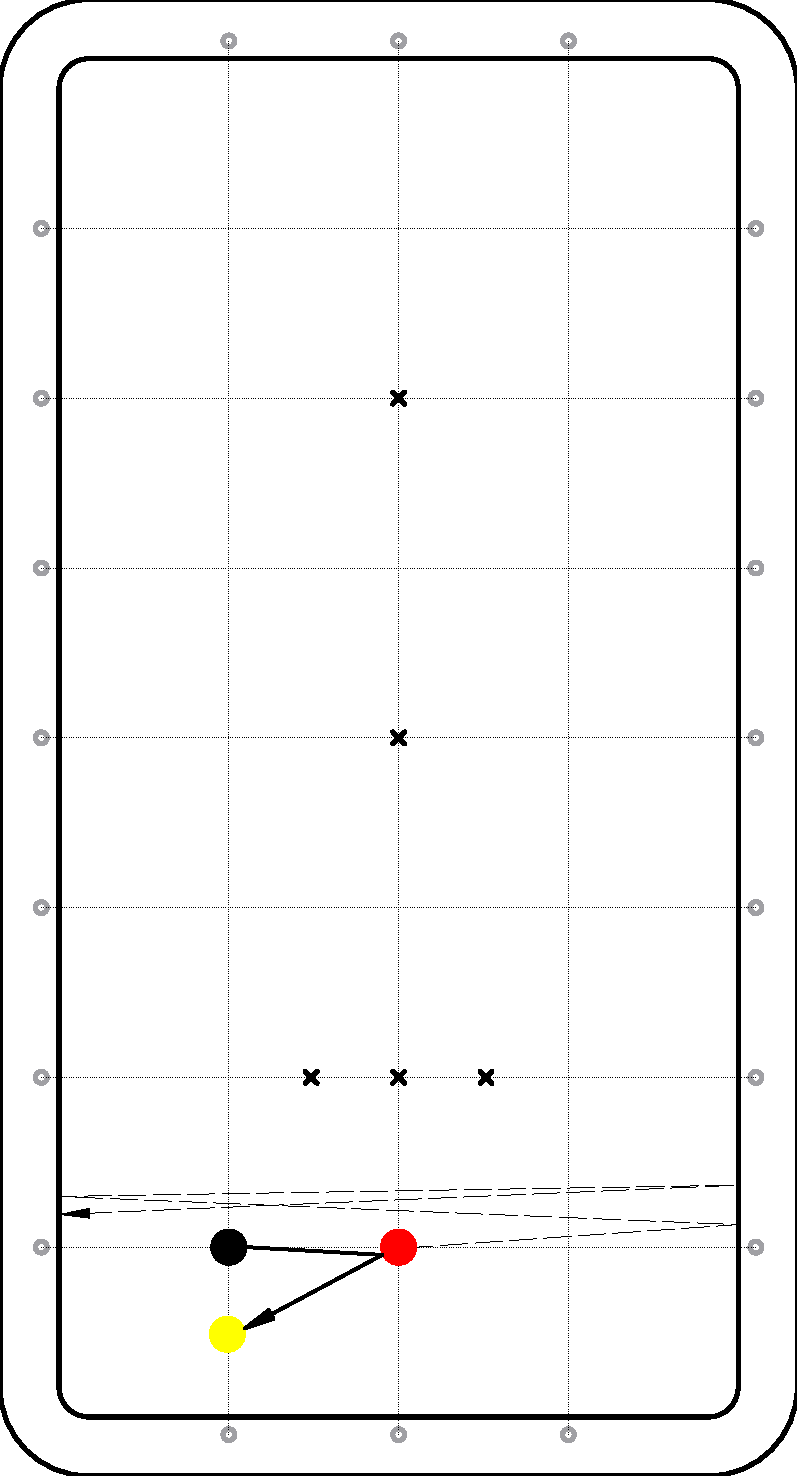
\includegraphics[width=0.85\linewidth]{B/imagesB/B11-01.pdf}
	\caption{Le r�tro qui double}
	\label{fig:B11-1}
\end{figure}

\clearpage
